\section{Resultate}
\label{sec:resultate}

Das optimierte Netz (Version v3) kommt mit 137 der ursprünglich 165 Visuren aus. Insgesamt wurden somit 28 Visuren
eliminiert. Die Anzahl der Beobachtungen nimmt dadurch in der Lage von 353 auf 297 und in der Höhe von 177 auf 150 ab.
\bigskip

Abbildung~\ref{fig:40_Optimiertes_Netz_Ägerdi_Brunni_Tal.png} und Abbildung~\ref{fig:41_Optimiertes_Netz_Sperre_Brichen.png}
zeigen das optimierte Netz mit den eliminierten Messungen. Der Grossteil der Visuren wurde im Gebiet Sperre entfernt,
wo die Querverbindungen zwischen den Stationen 1000, 2000, 210 und 510 sowie die Verbindungen 1000--2000 und 210--2000
vollständig weggefallen sind. Im Gebiet Brichen wurde vor allem die Station 7020 ausgedünnt, und die Verbindung
510--7020 entfällt. Im Gebiet Ägerdi und Brunni beschränken sich die Änderungen auf die Verbindungen 6003--6015 und
TP506--6001. Im Gebiet Tal wurden keine weiteren Visuren entfernt.

\bigskip
\begin{table}[H]
    \centering
    \small
    \setlength{\tabcolsep}{4pt}
    \begin{tabular}{@{}l cc cc cc cc@{}}
        \toprule
        & \multicolumn{2}{c}{v0} & \multicolumn{2}{c}{v1} & \multicolumn{2}{c}{v2} & \multicolumn{2}{c}{v3} \\
        \cmidrule(lr){2-3} \cmidrule(lr){4-5} \cmidrule(lr){6-7} \cmidrule(l){8-9}
        Kenngrösse & Lage & Höhe & Lage & Höhe & Lage & Höhe & Lage & Höhe \\
        \midrule
        \multicolumn{9}{@{}l}{\textit{Netz}} \\
        \quad Beobachtungen                    & 353 & 177 & 335 & 168 & 313 & 158 & 297 & 150 \\
        \quad Überbestimmungen                 & 189 & 112 & 171 & 103 & 149 & 93  & 133 & 85  \\
        \quad Entfernte Visuren (kumuliert)    & \multicolumn{2}{c}{0} & \multicolumn{2}{c}{9} & \multicolumn{2}{c}{20} & \multicolumn{2}{c}{28} \\
        \midrule
        \multicolumn{9}{@{}l}{\textit{Zuverlässigkeit}} \\
        \quad Beob. mit $z_i > 60\,\%$         & 160 & 104 & 135 & 93 & 98 & 82 & 80 & 66 \\
        \quad Beob. mit $z_i < 25\,\%$         & 37 & 4 & 37 & 4 & 41 & 4 & 40 & 4 \\
        \quad Unkontrolliert ($z_i = 0$)       & 22 & 9 & 22 & 9 & 22 & 9 & 22 & 9 \\
        \quad $|w_i|_{\max}$                   & 3.1 & 2.9 & 3.1 & 2.9 & 3.0 & 2.9 & 3.0 & 3.0 \\
        \midrule
        \multicolumn{9}{@{}l}{\textit{Genauigkeit}} \\
        \quad Quotient emp./theor. Gesamtnetz  & 0.86 & 1.02 & 0.89 & 1.01 & 0.93 & 1.01 & 0.96 & 1.01 \\
        \quad Mittlere Genauigkeit [mm]        & 1.7 & 2.1 & 1.7 & 2.1 & 1.8 & 2.1 & 1.9 & 2.2 \\
        \quad Schlechteste Genauigkeit [mm]    & 3.2 & 3.3 & 3.4 & 3.3 & 3.5 & 3.3 & 3.7 & 3.3 \\
        \quad\quad Punkt                       & TP510 & 6014 & TP510 & 6014 & TP510 & 6014 & TP510 & 6014 \\
        \quad Zweitschlechteste Genauigkeit [mm] & 2.6 & 3.0 & 2.7 & 3.0 & 2.8 & 3.0 & 2.9 & 3.0 \\
        \quad\quad Punkt                       & 6014 & 6013 & 6014 & 6013 & 6014 & 6013 & 6014 & 6013 \\
        \quad Drittschlechteste Genauigkeit [mm] & 2.2 & 2.9 & 2.3 & 2.9 & 2.4 & 2.9 & 2.5 & 2.9 \\
        \quad\quad Punkt                       & 6013 & 6002 & 6013 & 6002 & 6013 & 6002 & 6013 & 6002 \\
        \quad Punkte über Anforderung          & 2 & 0 & 2 & 0 & 2 & 0 & 2 & 0 \\
        \bottomrule
    \end{tabular}
    \caption{Kenngrössen der Ausgleichung über die Optimierungsschritte v0 bis v3. Genauigkeit = grosse Halbachse der Konfidenzellipse.}
    \label{tab:kenngroessen_optimierung}
\end{table}

Tabelle~\ref{tab:kenngroessen_optimierung} fasst die Entwicklung der Kenngrössen über alle Versionen zusammen.
Während die Anzahl der Beobachtungen mit hoher lokaler Zuverlässigkeit kontinuierlich abnimmt, bleibt die Anzahl
der unkontrollierten Beobachtungen in allen Versionen unverändert. Durch die Optimierung sind somit keine neuen
Schwachstellen im Netz entstanden. Keine normierte Verbesserung überschreitet den Grenzwert. Die Anforderungen 
an die Genauigkeit sind bis auf die Punkte TP510 und 6014 erfüllt. Diese überschreiten die
Lageanforderung bereits im Ausgangsnetz. Die Punkte 6013 und 6060 erreichen im optimierten Netz den Grenzwert.

\clearpage
\begin{figure}[H]
    \centering
    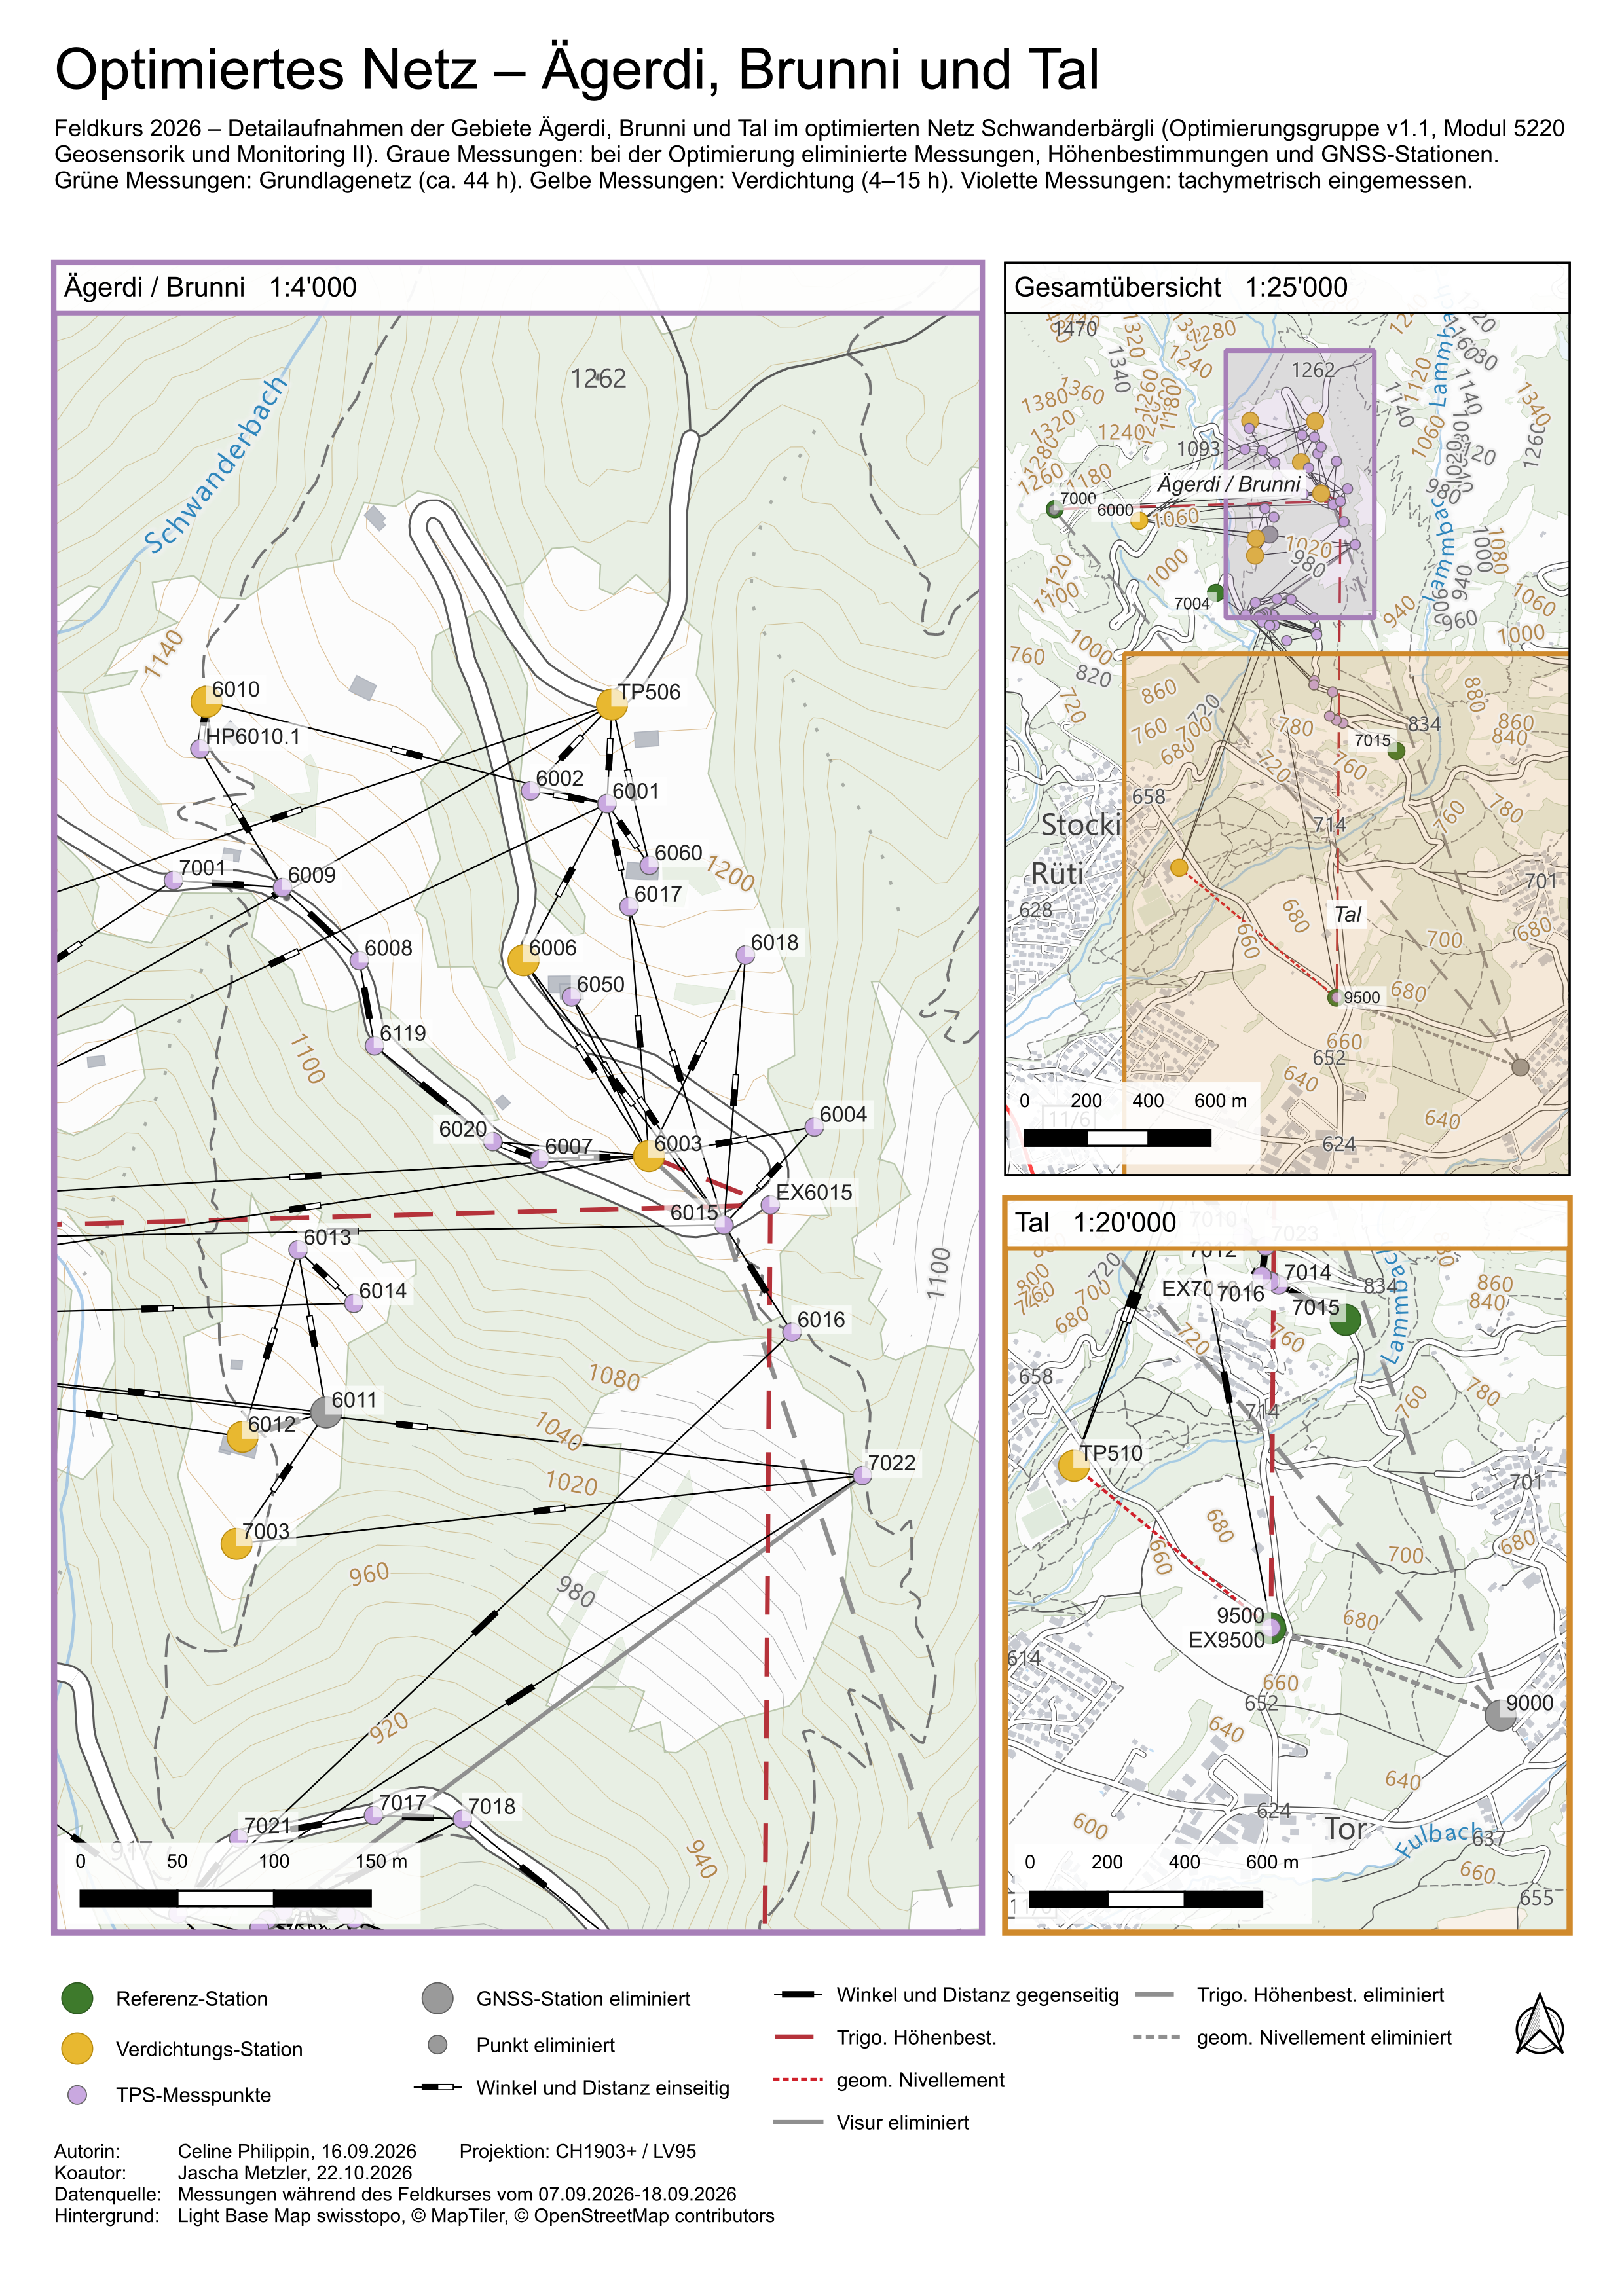
\includegraphics[width=\textwidth,
                     height=\dimexpr\textheight-4\baselineskip\relax,
                     keepaspectratio]{40_Optimiertes_Netz_Ägerdi_Brunni_Tal.png}
    \caption[Optimiertes Netz Ägerdi Brunni und Tal]{Detailübersicht der Gebiete Ägerdi, Brunni und Tal des Optimierten Netzes Schwanderbärgli 2026}
    \label{fig:40_Optimiertes_Netz_Ägerdi_Brunni_Tal.png}
\end{figure}
\clearpage

\clearpage
\begin{figure}[H]
    \centering
    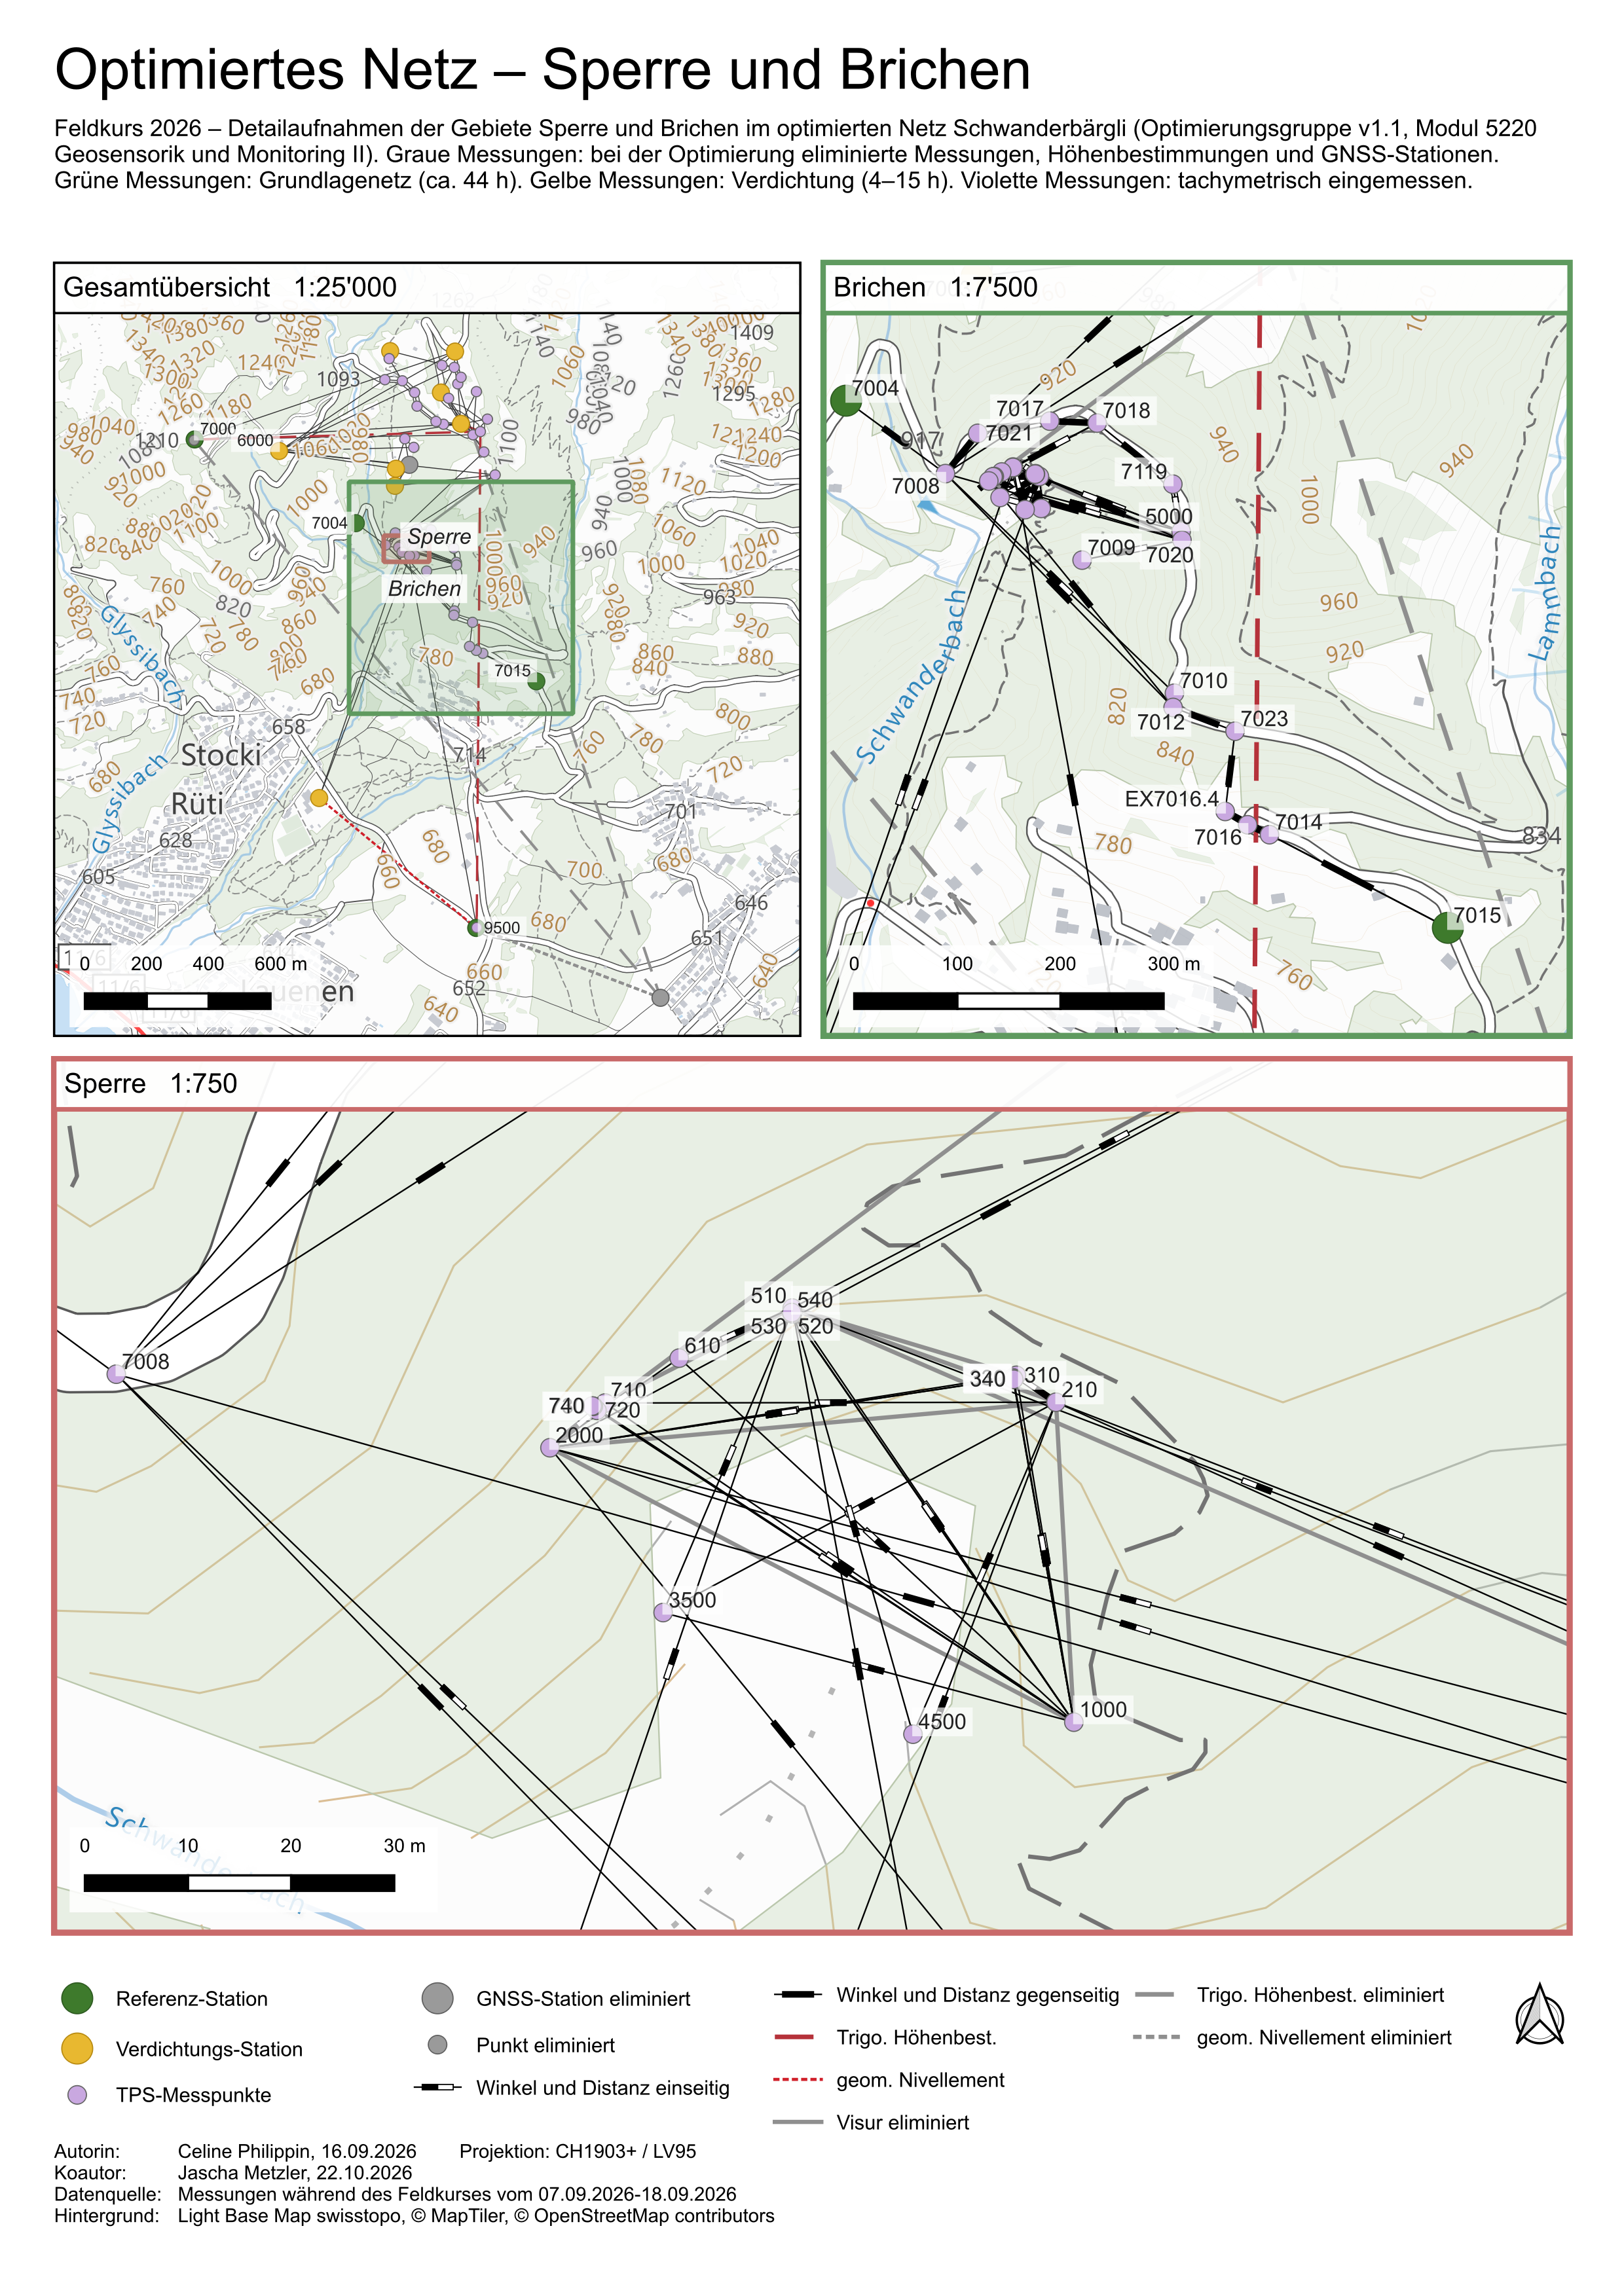
\includegraphics[width=\textwidth,
                     height=\dimexpr\textheight-4\baselineskip\relax,
                     keepaspectratio]{41_Optimiertes_Netz_Sperre_Brichen.png}
    \caption[Optimiertes Netz Sperre und Brichen]{Detailübersicht der Gebiete Sperre und Brichen des Optimierten Netzes Schwanderbärgli 2026}
    \label{fig:41_Optimiertes_Netz_Sperre_Brichen.png}
\end{figure}
\clearpage
\subsection{xxx}
\label{xxx}